\section{Explainable AI 3}
\subsection{Mutual information Neural Estimation (MINE)}
\subsubsection{KL-Divergence}
KL-Divergence
\[
D_{KL}(p||q) = \sum_{x} p(x) log \frac{p(x)}{q(x)}
\]
Is it a true metric?:
\begin{itemize}
    \item It is not symmetric\[
    D(p,q)  = D(p,q)
    \]
    \item Does not obey the triangle inequality\[
    D(q,r) \le D(p,q) + D(q,r)
    \]
\end{itemize}
Why define distance like this?
Defined in terms of information theory, not geometry.
Think of Q as been parametrized by a NN with params \(\theta\).
Blue distribution remains fixed Green must be optimized.

P is the true distribution of label.

Q is model distribution.

Forward KL is mean seeking.

Reverse KL is mode seeking.
\begin{figure}
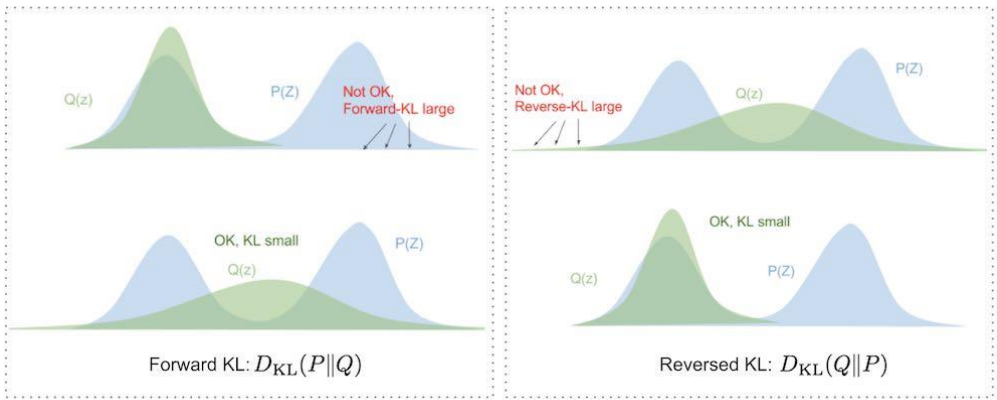
\includegraphics[width = \columnwidth]{figures/XAI3/KL.png}
\end{figure}

\subsubsection{Mutual Information}

MI is a special case of the KL-Divergence where the \(P=p(x,y)\) is given by the joint probability distribution and \(Q = p(x)p(y)\) is given by the product of the marginals.

The degree that the measured distribution differs from the baseline expected uncorrelated distribution is directly proportional to the MI
\begin{figure}[h!]
    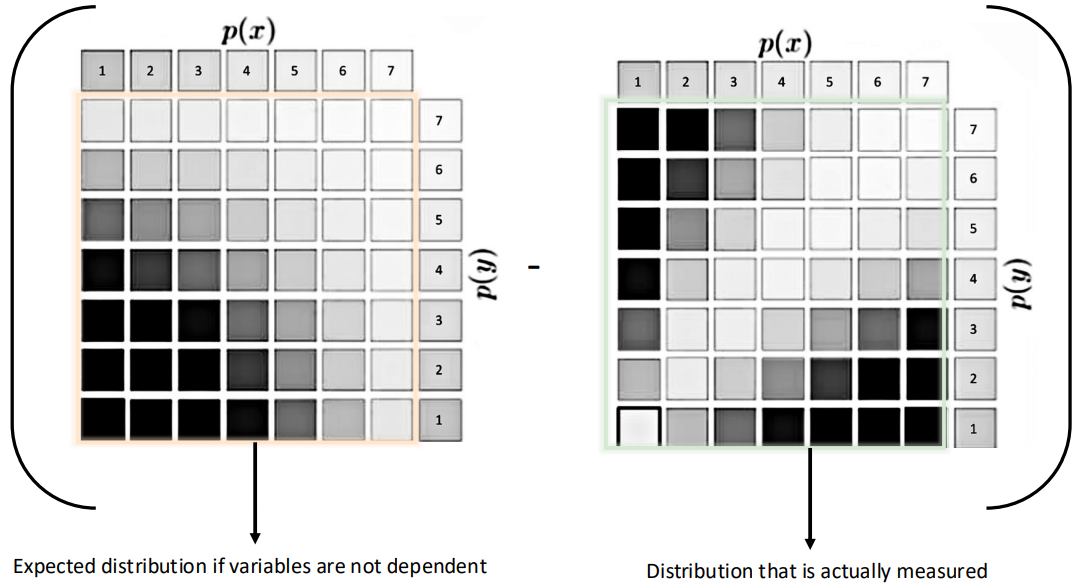
\includegraphics[width = \columnwidth]{figures/XAI3/MI.png}
\end{figure}
\[
MI(X;Y) = \sum_{x} \sum_{y} \colorbox{green!20}{$p(x,y)$} log \frac{\colorbox{green!20}{$p(x,y)$}}{\colorbox{orange!20}{$p(x)p(y)$}}
\]


\subsection{MINE-Network}
Use Deep learning to estimare MI in a dataset.
\subsubsection{Discreet}
Use K-means to cluster data.
K-means behaves like a multidimensional histogramm.
\begin{figure}[h!]
    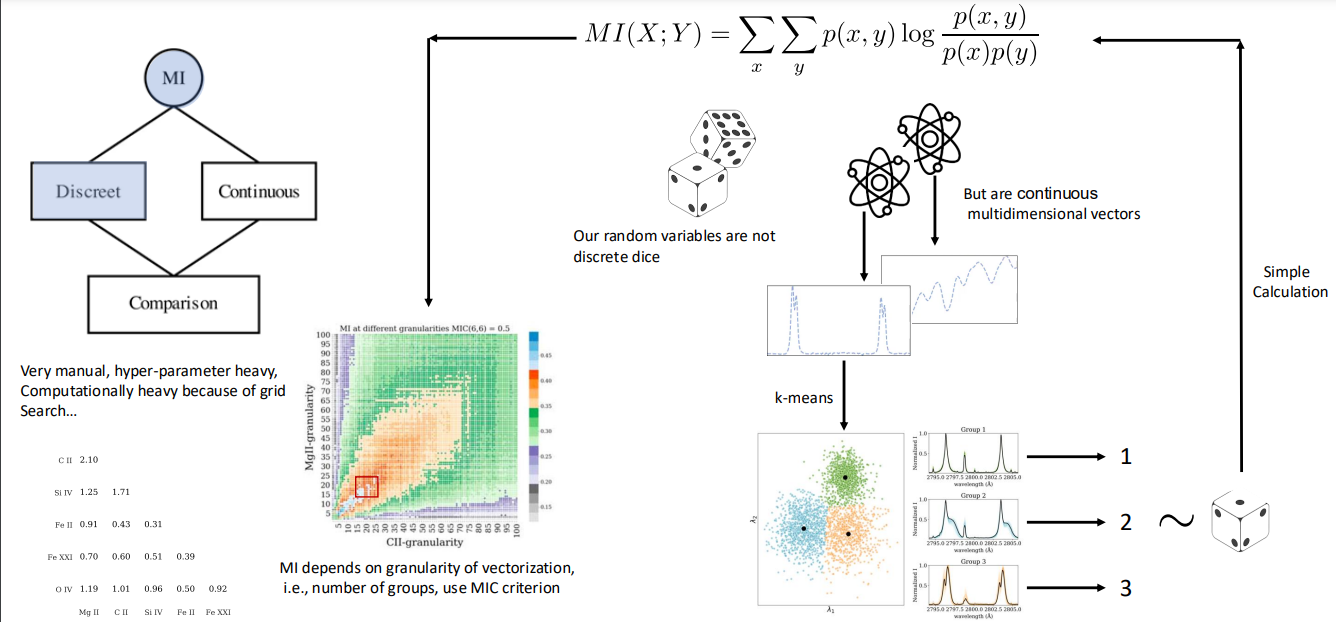
\includegraphics[width = \columnwidth]{figures/XAI3/DiscreetMINE.png}
\end{figure}

To derive the lower triangular matrix you require a huge amount of compute, to search all possible granularities to apply the MIC criterion!
\begin{itemize}
    \item Would be simple but the problem is that we do not have a closed form expression for the pdf's \(P\) and \(Q \)
    \item We can only sample from these distributions
\end{itemize}
\subsubsection{Continuous}
Use Neural Network istead of k-means.
\begin{figure}[h!]
    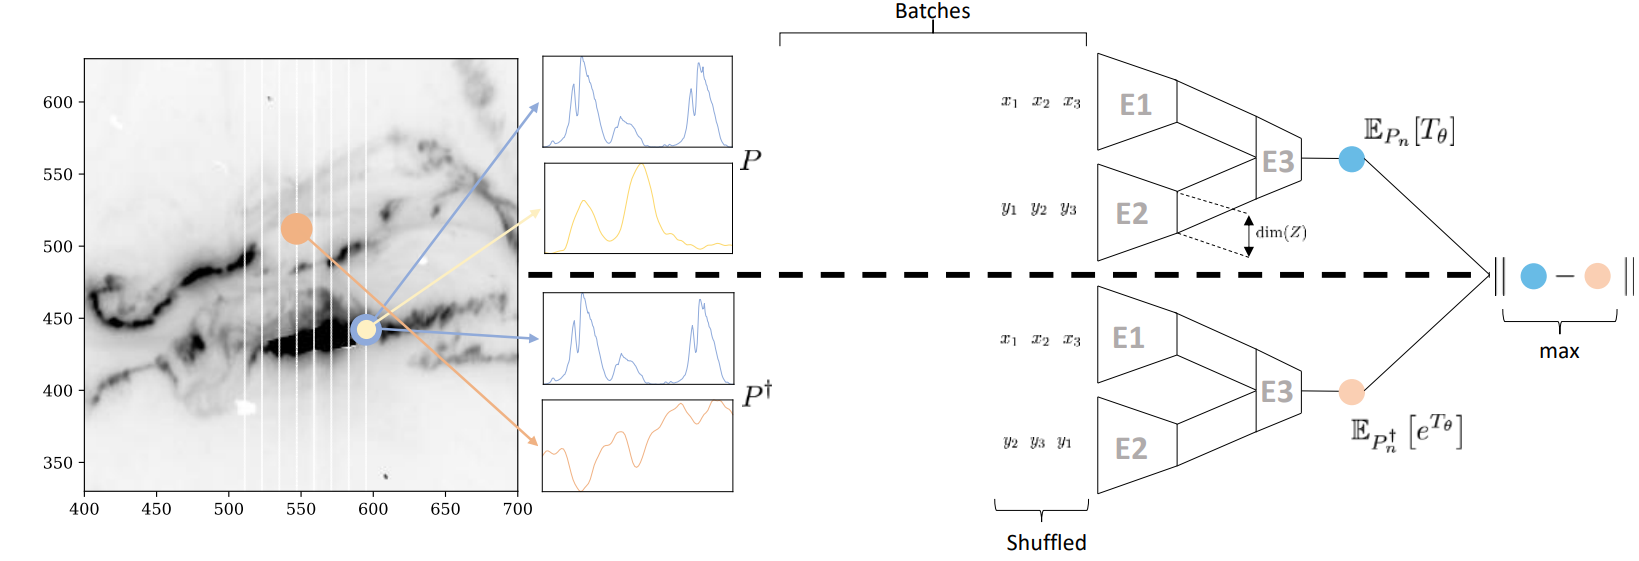
\includegraphics[width = \columnwidth]{figures/XAI3/ContinuousMINE.png}
\end{figure}

Upper part \(\mathbb{E}_{P_n}\left[T_\theta\right]\) represents green part of MI.

Lower part \(\mathbb{E}_{P_n}\left[e^{T_\theta}\right]\) represents orange part of MI.

\subsubsection*{Loss for network}
Donsker-Varadhan Representation of KL-Divergence
\[
D_{KL}(P||Q) = \sup_{T:\Omega \rightarrow \mathbb{R}}\mathbb{E}_P \left[T\right] - \text{log}(\mathbb{E}_Q\left[e^T\right])
\]
\(T:\Omega \rightarrow \mathcal{R}\): is a fucntion that takes in data of dimensions \(\Omega\) and maps to a real number

\(\sup\): Supremum means the function maximizes the expression over all measurable functions.

Allows us to turn the problem into a numercal optimization problem.

We can sample from the data and calculate the MI so long as we can find a function that is flexibke enough.

Applying the KL-Divergence to MI gives:
\[
MI(X;Y) = \sup_{T:\Omega \rightarrow \mathbb{R}}\mathbb{E}_{p(X,Y)} \left[T\right] - \text{log} (\mathbb{E}_{p(x)p(y)}\left[e^{T}\right])
\]
Parametrize,i.e., approximate the function T with a neural network
\[
MI_\Theta(X;Y) = \sup_{\Theta}\mathbb{E}_{p(X,Y)} \left[T_\theta\right] - \text{log} (\mathbb{E}_{p(x)p(y)}\left[e^{T_\theta}\right])
\]

We can estimate the expectations by sampling a large number of instances from the joint and product of the marginals.
\[
\mathbb{E}_{p(X,Y)}\left[T_\theta\right] \approx \frac{1}{N}\sum_{i = 1}^{N} T_\theta (x_i,y_i), \mathbb{E}_{p(X)p(Y)}\left[T_\theta\right] \approx \frac{1}{N}\sum_{i = 1}^{N} e^{T_\theta (x_i,y_i)}
\]

Our network objective function (Loss):
\[
\hat{MI}_{\Theta}(X;Y) = \frac{1}{N}\sum_{i = 1}^{N}T_\theta\underbrace{(x_i,y_i)}_{\text{same Pixel}} - log \left(\frac{1}{N}\sum_{i=1}^{N}e^{T_\theta\overbrace{(x_i,y_i)}^{\text{different Pixel}}}\right)
\]

\subsection{Shapley Values}
The problem:
\begin{itemize}
    \item If two fixes carry the same information and this information is critical for the modes prediction.
    \item Removing one pixel will not change the result because the load will be carried by the remaining pixel transmitting the same information
    \item The same is true for the other pixel
    \item Therefore, removing a single pixel at a time could result in the two most important feeatures being ranked as leased important. This is due to the coupling of pixel information, i.e., howdo features interact and correlate?
    \item  A mathematically exact way for calculating the contribution of each pixel/feature to the prediction is to sum over all possible subsets of pixels\dots
    \item This means \(2^n\) combinations (each is on or off and n pixels), for a small colour image \(2^786432\) unique subsets\dots
\end{itemize}

\subsubsection{The optimal solution}
\begin{figure}[!h]
    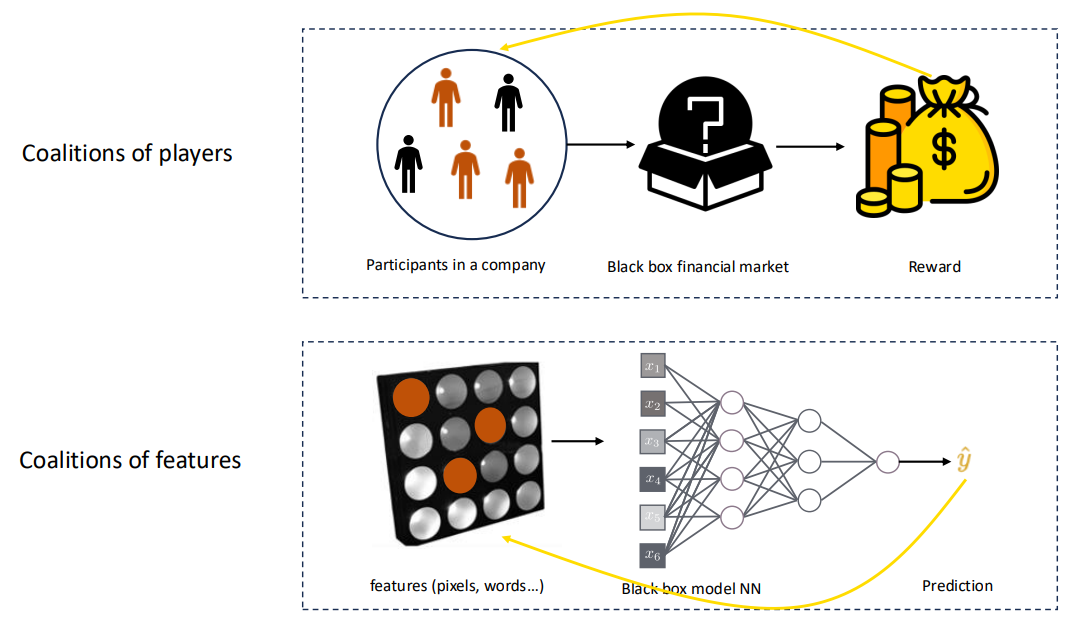
\includegraphics[width = \columnwidth]{figures/XAI3/ShapleyValuesGameTheory.png}
\end{figure}
\subsubsection{The maths}
The reward/importance of the \(i\)'th person/feature is the average marginal contribution of feature \(i\) across all possible subsets, weigthed by the probability of each subset occuring.
This is called \textbf{feature Shapley Values}

\[
\phi_i(x) = \colorbox{yellow!20}{$\sum_{S \subseteq N \setminus{i}}$} \colorbox{red!20}{$\frac{|S|! \times \left(|N|- |S|-1\right)!}{|N|!}$}\colorbox{green!20}{$\left(f_\theta (S \cup \left\{i\right\})-f_\theta (S)\right)$}
\]
\(|S|\) = Size of subset

\(|N|\) = Total number of features

\(|N|-|S|-1\) = Number of features not in \(S\) excluding \(i\)
\begin{itemize}
    \item \colorbox{red!20}{Red}: Probability of obtaining each subset \(S\) when randomly selecting features
    \item \colorbox{yellow!20}{Yellow}: Sum over all subsets of total \(N\)
    \item \colorbox{green!20}{Green}: Difference between model prediction with and without feature \(i\)
\end{itemize}
Normalization factor is important otherwise sets that are small or close to \(N\) would contribute less since their are fewer subsets of these sizes.
\begin{itemize}
    \item \textbf{Effciency} (or Addivity): The sum of all the Shapley values equals the total prediction of the model when all features are included.
    \[
    \sum_{i = 1}^{n} \phi_i(v) = f(N)
    \]
    \item \textbf{Symmetry}: If two features contribute equally to all possible coalitions, their Shapley values should be equal.
    \[
    \text{If \(f(S\cup i) = f(S \cup j)\)  then \(\phi_i(f) = \phi_j(f)\)}
    \]
    \item \textbf{Dummy} (or Null Player): If a feature adds no marginal value to any coalition, its Shapley value should be zero.
    \[
    \text{If \(f(S\cup i) = f(S)\)  then \(\phi_i(f) = 0\)}
    \]
    \item \textbf{Linearity}: The Shapley value of a sum of two games should be the sum of the Shapley values of the individual games. This allows for decomposition of complex games into simple ones.
    \[
    \phi_i(f+g) = \phi_i(f) + \phi_i(g)
    \]
\end{itemize}
\subsubsection{The problem}
Network requires information to run through, need good baseline to represent missingness.
\subsubsection{Monte Carlo approximation}
\begin{figure}[!h]
    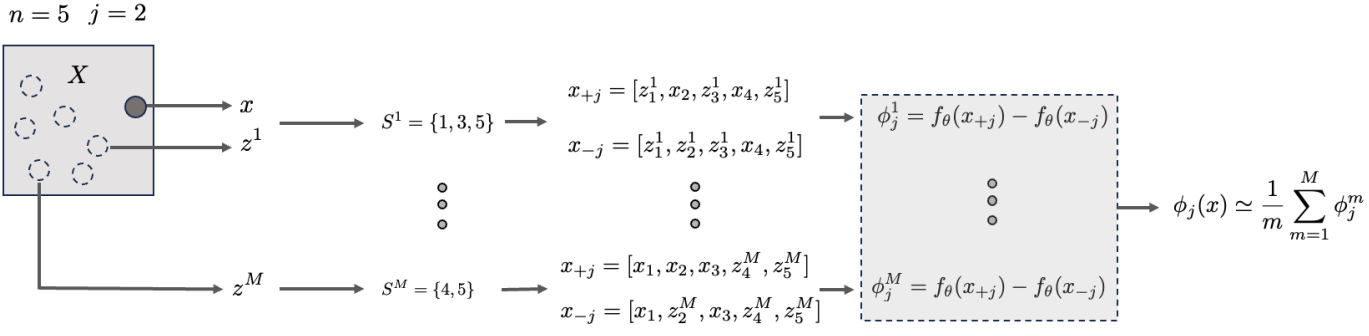
\includegraphics[width = \columnwidth]{figures/XAI3/ShapleyValuesMonteCarlo.png}
\end{figure}
\begin{itemize}
    \item Approxmate missingness by using random features from random samples as background
    \item Value with and without
    \item Normalization simpler because sample from a flat distribution,i.e.,ever combination is equally probable
\end{itemize}
Why do we only use the background from a single instance of a time and don't mix the z's from different instance?:
To reduce the production of unrealistic data

\subsubsection{Expected Gradients | Image data}
Problem: each baseline comes with a bias

Solution: Shapley value treatment in image space
\begin{itemize}
    \item An additional integral over multiple image paths
    \item We sample from the dataset
    \item We take the expectation because the integral is intractable
\end{itemize}
\begin{figure}[!h]
    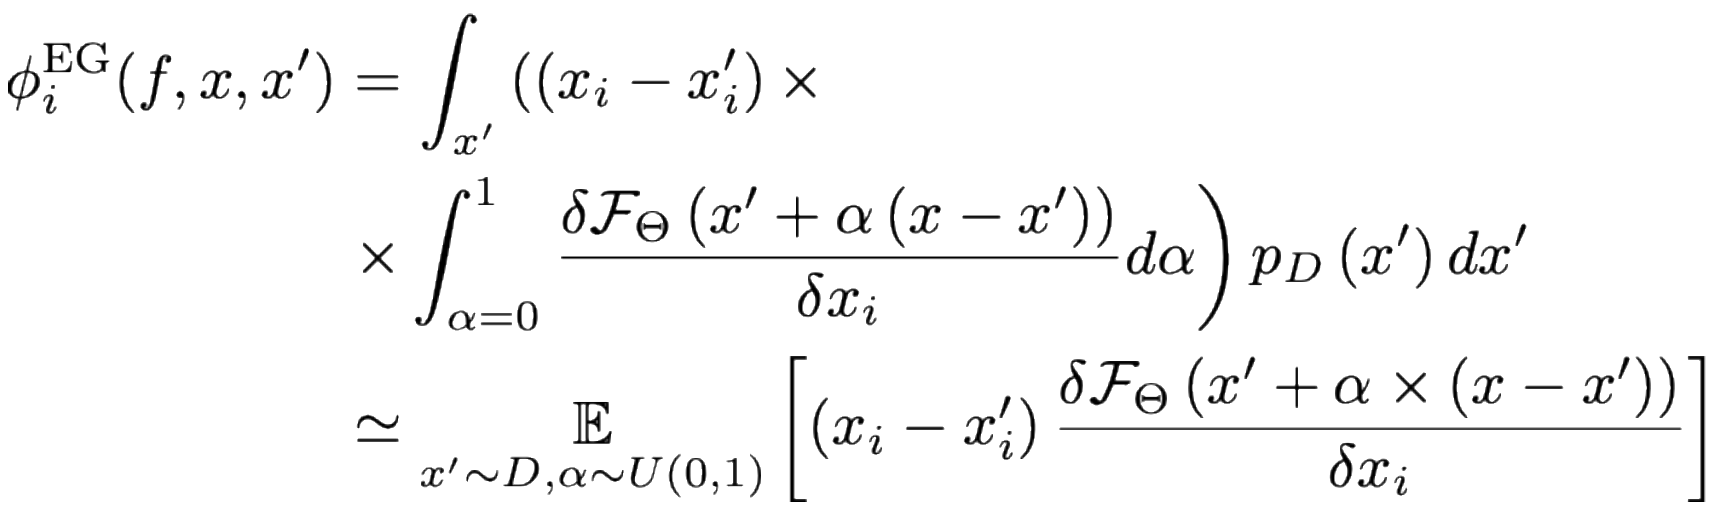
\includegraphics[width = \columnwidth]{figures/XAI3/ShapleyValuesXGRADFromula.png}
\end{figure}
\subsubsection*{Example}
\begin{enumerate}
    \item Start from baseline (blue)
    \item Linearly Interpolate to target, i.e., different pathes to same (orange)
    \item Calculate accumulated grads along each path for each wavelength
    \item Expectation value instead of intractable integral
    \item Create heatmap from pixel/wavelength attributions
    \item Require a background dataset (500 randomly sampled spectra)
\end{enumerate}
\begin{figure}[!h]
    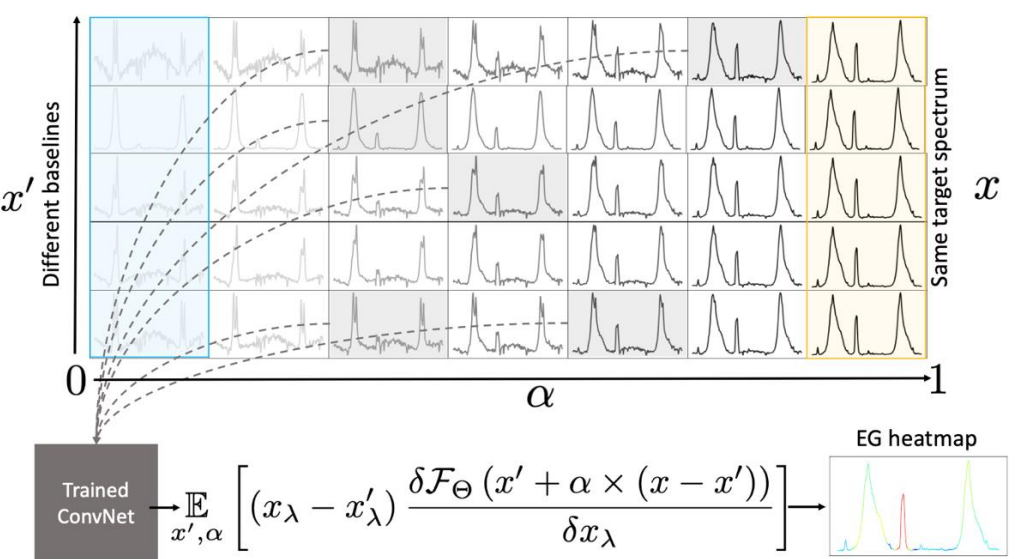
\includegraphics[width = \columnwidth]{figures/XAI3/ShapleyValuesXGRADExample.png}
\end{figure}
\begin{itemize}
    \item An additional integral over multiple image paths
    \item We sample from the dataset
    \item We take the expectation because the integral is intractable
\end{itemize}
We don't want to see the affects of our baseline on the models output.
All the other baseline biased the result (black, white, blur), even the gaussian noise assumes pixels are uncorrelated.
By using the background dataset as a baseline, we ensure that we resepct the dependencies between the pixels.
Additionally, integrating along many image paths against this background ensures that in the limit, the baseline leaves the output stationary with respect to the models average prediction, since some feature will fight to increase the models prediction, while others try to decrease it.
This implies that the additional integration over mulitple image paths is an effective way to take pseudo subsets, i.e., the additional integral allows is to effectively turn features on and off wihtout introducing bias into our explanation.

Features:
\begin{itemize}
    \item Obeys mathematical axioms
    \item Model agnostic
    \item Can solve XOR 
    \item Robust to hyperparameters
    \item Data agnostic
\end{itemize}
Problems:
\begin{itemize}
    \item Requires background dataset
\end{itemize}

\subsection{Local model agnostic}